\subsection{Raaum's BusTUC Android Application}

BusTUC Android Application is the application that was created by Magnus Raaum\cite{mag}. It displays a map with user and bus stop locations, and an input field for entering the desired destinations. The system uses the closest bus stops to a user's location to search for possible routes, by sending queries to BusTUC. Received departure suggestions are then updated with real-time departure times, before they are shown to the user as plain text suggestions.

\subsection{Existing Solutions in Trondheim}
\label{sec:existingtrondheim}
The following sections describe existing applications, developed for getting info about bus transportation in Trondheim. 
\begin{table}[!h]
\label{tab:funcintest}
\begin{center}
   \caption{Functionality in the tested applications.}
    \begin{tabular}{ |  l  |  l  |  l  |  l  |  l  |  }
    \hline
    Application & Bartebuss & Alf's Bybuss & Bussdroid & Busstider\\ \hline
    Bus oracle & Yes & Yes & Yes & Yes \\ \hline
    Map & Yes  & Yes & No & Yes \\ \hline
    Favourites & Yes & No & No & No \\ \hline
    History & Yes & Yes & Yes & No \\ \hline
    Real-time & Yes & Yes & Yes & No \\ \hline
    \end{tabular}
\end{center}
\end{table}
Table \ref{tab:funcintest} gives a summarised comparison of the tested applications. Below a brief description of each criteria is given. The following sections describe all the tested applications.
\\\\
\newpage
\begin{description}
\item [BusTUC]
Whether the tested application uses BusTUC as a functionality
\item [Map]
Whether the tested application integrate maps
\item [Favourites]
Favourites functionality allows a user to store queries or specific bus stops for later use. A typical usage is to store a query with an additional tag
\item [History]
History defines earlier searched queries or selected bus stops, stored in the internal or the external storage
\item [Real-time]
Whether the tested applications provide real-time data.
\end{description}

\subsubsection{Bartebuss}
\label{sec:bartebuss}
\emph{Bartebuss}\footnote{http://bartebuss.no/om} is developed in HTML5 by Rune M. Andersen,  and uses the \emph{BusBuddy} API\footnote{http://busbuddy.norrs.no/}. It has rich functionality, with options to store favourites, find near-by bus stops, search for specific bus stops, use BusTUC and show maps. Due to the use of HTML5, the map is not as responsive as in a native application. The user interface on the other hand is intuitive and easy to navigate but it might provide too many choices to the user.
\setlength{\intextsep}{0pt}
\begin{wrapfigure}{l}{0.5\textwidth}
  \begin{center}
    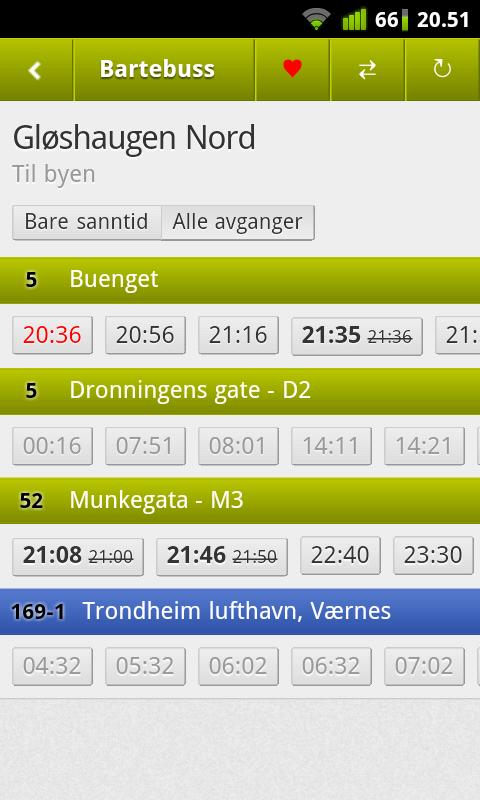
\includegraphics[scale=0.25]{ExistingSolutions/bartebuss.jpg}
  \end{center}
  \caption{Bartebuss}
\end{wrapfigure}
\setlength{\intextsep}{3pt}
There are 5 ways to use the application to find bus departures. The first is through ''favourites'', where several bus stops can be stored(giving quick access). When a favourite is selected, real-time data for the bus stop is displayed. The second way to use the application is an option called ''near me'', where the closest bus stops to a user's location are listed. Items can be selected the same way as in favourites. The third option is ''search''. Here, the user can search for a specific bus stop, and view real-time data. The fourth option is BusTUC, where a text field is used for query input. The last option is to select a bus stop icon from the map, which triggers a rewrite of real-time data. The map part was lagging during testing on the Android platform, and hardly usable at all. Two other problems are the lack of pinch zooming and poor handling of landscape/portrait changes(as resizing causes problems). When tilted to landscape mode, the zoom controls disappear.

\subsubsection{Alf's ByBuss}
\emph{Alf's ByBuss} \footnote{http://bybuss.alfsimen.com} is a native Android application, developed by Alf Simen S\o rensen. It also uses the \emph{BusBuddy} API. It has a simple user interface, and provides BusTUC functionality, with the option to include the user's location as the departure parameter.
The application has a text field for entering queries, and some additional functionalities in the menu (activated by the menu button). The main component of the user interface is a map showing clickable bus stop icons. The user can select the bus stop icons, with corresponding bus stop names, as departure and destination, and view real-time data. Menu options include: ''Use my existing location''(which inserts the user's current location into the text field as departure input), ''reverse search''(which switches the departure and destination stops), and a link to the online bus schedules. \emph{Alf's ByBuss} appears more responsive than \emph{Bartebuss} during map navigation, but the user interface is not as polished. 
\subsubsection{Bussdroid}
\emph{Bussdroid} \footnote{market.android.com/details?id=com.ken.bussdroid} is a native Android application by Ken B\o rge Viktil. Unlike the two previously tested applications, it does not provide a map. The functionality consists of real-time data for bus stops, a BusTUC query text field and the possibility to store queries as favourites. The application is responsive, and has a clean and intuitive user interface. 

\subsubsection{Busstider}
\emph{Busstider} \footnote{http://www.a2bsoft.net/projects/busstider} is a native Android application by Martin M. Syvertsen. Functionality is limited to BusTUC, and a map displaying bus stop icons. Real-time data is not available. There are two ways to use the application: 1) Asking BusTUC with a natural language query, 2) selecting departure and destination by clicking icons on the map. It has a simple and intuitive user interface based on tabs, and is fairly responsive.
\begin{figure}[!h]
\begin{tabular}{ccc}
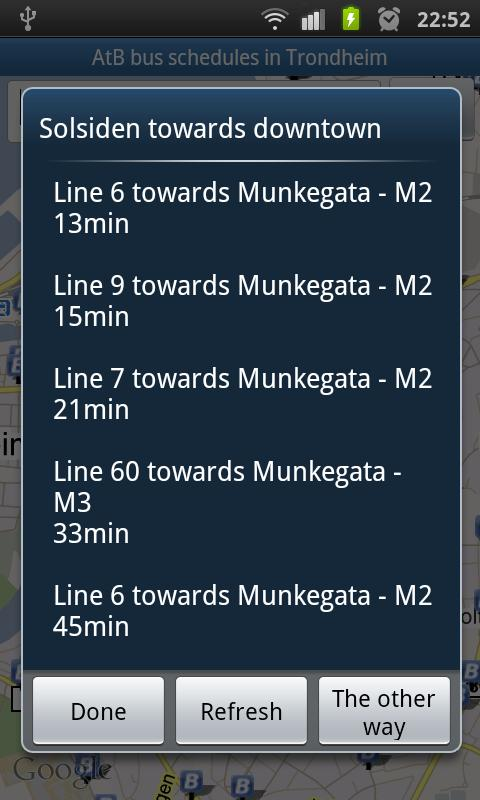
\includegraphics[width=0.27\linewidth]{ExistingSolutions/alfsbybuss.jpg} & 
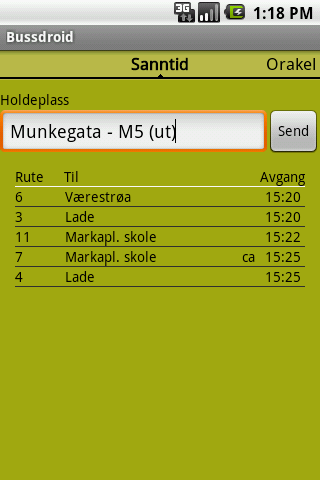
\includegraphics[width=0.27\linewidth]{ExistingSolutions/bussdroid.png} &
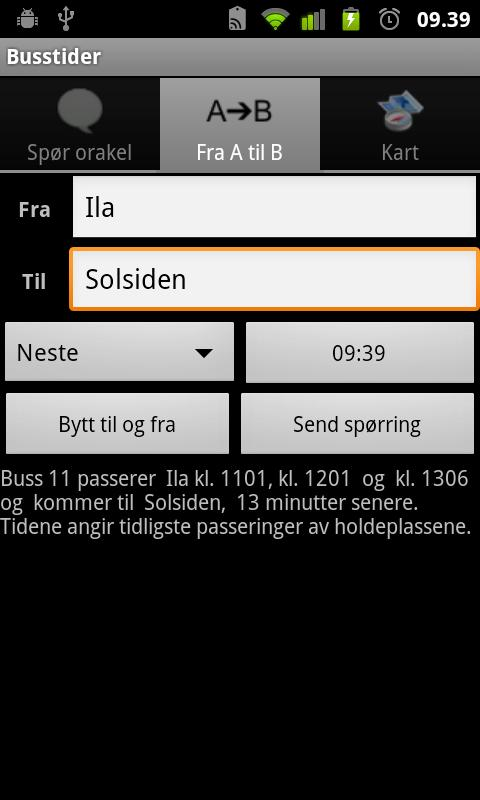
\includegraphics[width=0.27\linewidth]{ExistingSolutions/busstider.jpg}\\
\end{tabular}
\caption{From left to right: (1)Alf's ByBuss, (2)Bussdroid, (3)Busstider}
\end{figure}
\newpage
\subsubsection{BusBuddy API}
\emph{BusBuddy}\footnote{http://api.busbuddy.no/} is an API developed by Roy Sindre Norangshol, aimed at the retrieval of real-time data. It is a hobby project with the goal to minimise the overhead of SOAP messages downloaded to the mobile devices. Both \emph{Bartebuss} and \emph{Alf's ByBuss}, use this API. All applications developed with the \emph{BusBuddy} API are available through GIT Hub\footnote{https://github.com/}, as \emph{BusBuddy}'s policy is that development projects should be open source. 

In the early stages of the project using this API was considered . However, the disadvantages lead to discarding of the idea. As it is a hobby project, retrieving a license key was not easy. In addition, \emph{BusBuddy}'s username and password for access to AtB's real-time system is not permanent. AtB can retract this at any time. The process of retrieving new keys, would have to go through the \emph{BusBuddy} crew. By using the username and password provided by LingIT, this ``middle man'' operation is avoided. It is also likely that AtB would renew the username and password quicker for LingIT, than for a private operator.

\subsubsection{Summary of Existing Solutions in Trondheim}
All the tested applications for bus route information in Trondheim are already downloaded by several users, indicating that they have attractive functionalities. For our project it was important to investigate what has to be done to move the concept of a bus route information application to a new level. And also to compare the different levels of artificial intelligence in the apps. 

Especially \emph{Alf's ByBuss} and \emph{Bartebuss} are close to our goals: they use BusTUC, maps and real-time functionality. Both \emph{Alf's Bybuss} and \emph{Bartebuss} integrate natural language through BusTUC, but aside from this, they do not have any other functionalities involving artificial intelligence. Their functionalities are based only on user input and menu navigations. The main topic of our project is reducing user input. In Raaum's application, route suggestions were calculated based on the closest stops to the user's location, and were automatically updated with real-time departure times. This is the core of the development of TABuss. Though the display of real-time data when a user presses a bus stop icon is an important functionality, we have to keep in mind the artificial intelligence aspects. This can separate our project from \emph{Alf's ByBuss} and \emph{Bartebuss}, and give us an upper hand regarding market potential.

\subsection{Extended Research}
Even though there are several applications available in Trondheim for bus route information, an expanded view including other cities and research performed is more informing. As discussed in Section \ref{sec:existingtrondheim}, aside from the general use of BusTUC, no functionalities in the tested applications can contribute to moving TABuss forward in the field of artificial intelligence. This section describes research areas within bus route information systems, with the main focus on intelligence through natural language, and the use of real-time data. 

\subsubsection{Natural Language Applications}
In intelligent route information systems, natural language has been addressed by different reseach papers\cite{Raux03let'sgo:}\cite{Turunen_mobilespeech-based}\cite {Turunen_designof}\cite{Turunen06evaluationof}. 

Raux et al.(2003) developed a system called \emph{Let's go}, which uses speech through phone calls as input, for returning route information\cite{Raux03let'sgo:}. The system was developed for ''elderly and non-native English speakers'', and provided information for the city of Pittsburgh. Speech was recognised by comparison and retrieval of the closest match. Emphasis was on creation of a grammar model for spoken language, and to include an overall generality regarding different structuring of sentences with the same meaning. Through their work, Raux et al. identified several challenges with speech processing and route information. The main challenge was that different users structured the same phrases differently, when referring to bus stops or places. Hypothetically, assuming BusTUC has a similar up to date speech system (\emph{TeleBuster}\footnote{http://www.idi.ntnu.no/~tagore/telebuster/} is not in use), this system would have to be able to infer correct mappings from spoken text, and also be able to extract content from text spoken with different dialects. As Trondheim is a city with inhabitants from different areas of Norway, this could become a complex operation. 

Turunen et al. (2007)\cite{Turunen_designof} (2006)\cite{Turunen06evaluationof} proposed a similar solution, \emph{TravelMan}, developed for the city Tampere in Finland. \emph{TravelMan} is an updated version of \emph{StopMan}\cite{Turunen_mobilespeech-based}(2006), which provided route planning. Input consisted of locations or addresses, provided to the system by text or speech. The user could also set personal preferences, such as exclusion of transportation options, as \emph{TravelMan} in addition to bus transportation, covered metro and tram. Of other features, a guidance functionality for visually impaired users was implemented, to provide what was referred to as an ''unbroken trip chain''. An unbroken trip chain was a successful trip, completed with full system guidance.


An interesting feature in \emph{TravelMan} related to our project, is the use of context and user location. The real-time guidance relies on location information, which also could be used to infer departure addresses. 
A video of TravelMan in use is available at YouTube \footnote{http://www.youtube.com/watch?v=bPVAQtHtC3s}

\subsubsection{Real-time Bus Information}
Early research focused on finding an optimal route. The Traveling Salesperson Problem \cite{tsp} is transferrable to route information, and several algorithms have been proposed. An example is Robert J. Szczerba et al.'s (2000) paper, which described an adaptation of the A*\cite{astar} algorithm, for finding the optimal route in real-time\cite{szc}. Assuming bus route companies incorporate a similar feature when planning routes, an algorithm including traffic information could give a real-time estimate of where the bus is at a given time. 

Maclean and Dailey's \emph{MyBus}(2000) predicts real-time arrival of buses by using historical data, the bus schedule and an prediction algorithm\cite{mybus}. This algorithm, based on Kalman filters \cite{kalman}, produced estimates, where traffic and passenger information is used as noise, affecting the original schedule.

Maclean and Dailey also published an article on a \emph{Mobile MyBus}(2001), which used communication through WAP\cite{maclean}. This system gave users real-time information based on received input. The input consisted of destination and a route number, sent by a URL request, and forwarded to the \emph{MyBus} server. Both were provided as digits as devices at that time did not have any input mechanism similar to a computer keyboard. In our project, this functionality can be compared to retrieving a real-time ID for a bus stop, before sending a SOAP-request to fetch real-time data. 

\begin{wrapfigure}{l}{0.5\textwidth}
  \begin{center}
    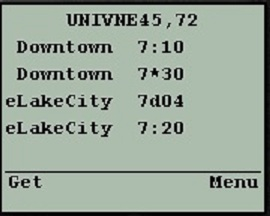
\includegraphics[scale=0.8]{ExistingSolutions/mybus.jpg}
  \end{center}
  \caption{MyBus WAP}
\end{wrapfigure}

Today, buses have GPS-trackers on-board, transmitting location information to a server. Real-time data is updated at specific time intervals and is fairly accurate. The real-time service was introduced in Trondheim by AtB. A similar service is provided in Oslo\footnote{http://trafikanten.no/}.

Ferris, Watkins and Borning's \emph{OneBusAway}(2010)  \footnote{www.onebusaway.org} focuses on context awareness in addition to the use of real-time data\cite{Onebusaway}. \emph{OneBusAway} uses the location of the user to automatically display the closest bus stops on a map, similar to TABuss. Context aware functionality proved to be successful through user testing, where 93 per cent of the existing users of \emph{OneBusAway} reported that more concise information was provided.

What differs \emph{OneBusAway} from TABuss, is that TABuss' main query functionality only needs the users destination as input. \emph{OneBusAway} needs to know both the departure stop and which route to select in order to reach planned destination. 


\subsubsection{Summary of Extended Research}
Both \emph{TravelMan} and \emph{Let's Go} utilise speech recognition to provide route information.\emph{TravelMan} extended the concept even further by introducing real-time guidance based on user location, and had features worth researching for future functionality. It was shown through Turunen et al.'s work that natural language has potential for mobile development and route information applications. 

BusTUC has since its release become a popular choice in Trondheim. As users have become familiar with the usage of natural language, a logical next step could be to introduce speech. iPhone 4S has implemented a system called SIRI\footnote{http://www.apple.com/iphone/features/siri.html}, which also contributes to familiarising people with natural language.

Research on the usage of real-time information has shown progress; from using estimated real-time, to actual real-time data. Maclean and Dailey's \emph{MyBus} WAP version was used over 9000 times, in a time period between its release in September 2000-January 2001, giving an indication that real-time route information on mobile devices is a promising field.
